\documentclass[aspectratio=169,10pt]{beamer}

% ==========================================================
% superdeck_v2.tex — Master research narrative deck
% TU/e 30 min  vs  TUM 60 min via \longtrue toggle.
%
% Dominant thesis:
%   Scheduling in business processes is fundamentally non-local.
%   Local dispatching rules and naive learning objectives fail once
%   uncertainty, calendars, downstream costs, and synchronization are present.
%
% Markers:
%   % CORE     always shown
%   % EXPAND   show for 60 min version
%   % APPENDIX backup / deep math
% ==========================================================

% ---- Talk-length toggle ----
\newif\iflong
\longfalse      % TU/e (30 min)
% \longtrue     % TUM (60 min)

% ---- Theme ----
\usetheme{Madrid}
\usecolortheme{beaver}
\setbeamertemplate{navigation symbols}{}
\setbeamertemplate{footline}[frame number]
\setbeamerfont{title}{series=\bfseries}
\setbeamerfont{frametitle}{series=\bfseries}

% ---- Packages ----
\usepackage[T1]{fontenc}
\usepackage[utf8]{inputenc}
\usepackage{graphicx}
\usepackage{booktabs}
\usepackage{amsmath,amssymb}
\usepackage{mathtools}
\usepackage{xcolor}
\usepackage{tikz}
\usetikzlibrary{arrows.meta,positioning,shapes.geometric,calc,fit}
% beamer loads hyperref; don't re-load it here (avoids option clash)

% ---- Figures in repo ----
\graphicspath{
  {Business_Process_Optimization/figs/}
  {ICAPS_problem_definition_final/images/}
  {IJCAI2026_Learn_to_Schedule/}
  {IJCAI2026_Learn_to_Schedule/new_plot/}
}

% ---- Colors / helpers ----
\definecolor{darkred}{RGB}{140,0,0}
\definecolor{darkgray}{RGB}{60,60,60}
\definecolor{okblue}{RGB}{31,119,180}
\definecolor{okgreen}{RGB}{44,160,44}
\definecolor{okorange}{RGB}{255,127,14}
\definecolor{badred}{RGB}{214,39,40}
\newcommand{\btext}[1]{\textbf{\color{darkred}#1}}
\newcommand{\smallref}[1]{{\scriptsize\color{darkgray}#1}}

% ---- Section slide ----
\AtBeginSection[]{
  \begin{frame}{Narrative spine}
    \tableofcontents[currentsection,hideothersubsections]
  \end{frame}
}

% ==========================================================
% Title
% ==========================================================
\title[Structure-Aware BPO Scheduling]{Structure-Aware Scheduling in Business Processes:\\From Proactive Planning to Valuation-Aware Control}
\author[Arik Senderovich]{Arik Senderovich}
\institute[York University]{York University}
\date{January 2026}

\begin{document}

% CORE
\begin{frame}
  \titlepage
  \vspace{-0.25cm}
  \begin{center}\small\color{darkgray}
    \iflong
      Technical University of Munich
    \else
      Eindhoven University of Technology
    \fi
  \end{center}
\end{frame}

% CORE
\begin{frame}{Thesis: scheduling in business processes is fundamentally non-local}
  \begin{block}{Claim}
    Local dispatching rules, naive learning objectives, and ``fair'' heuristics fail once
    \btext{uncertainty}, \btext{calendars}, \btext{downstream costs}, and \btext{synchronization} are present.
  \end{block}
  \vspace{0.15cm}
  \begin{block}{What replaces them}
    \btext{Structure-aware decision making:}
    robust proactive planning (BPSP) \(\rightarrow\) decision-aware learning (SASS) \(\rightarrow\) valuation \& incentives (capstone).
  \end{block}
  \vspace{0.2cm}
  \smallref{Framing background: Dumas et al., \emph{Fundamentals of Business Process Management}, 2nd ed., 2018.}
\end{frame}

% ==========================================================
% 1) BPO as high-stakes decision making
% ==========================================================
\section{BPO as high-stakes decision making (running example: DayHospital)}

% CORE
\begin{frame}{BPO turns process models into operational commitments}
  \begin{center}
    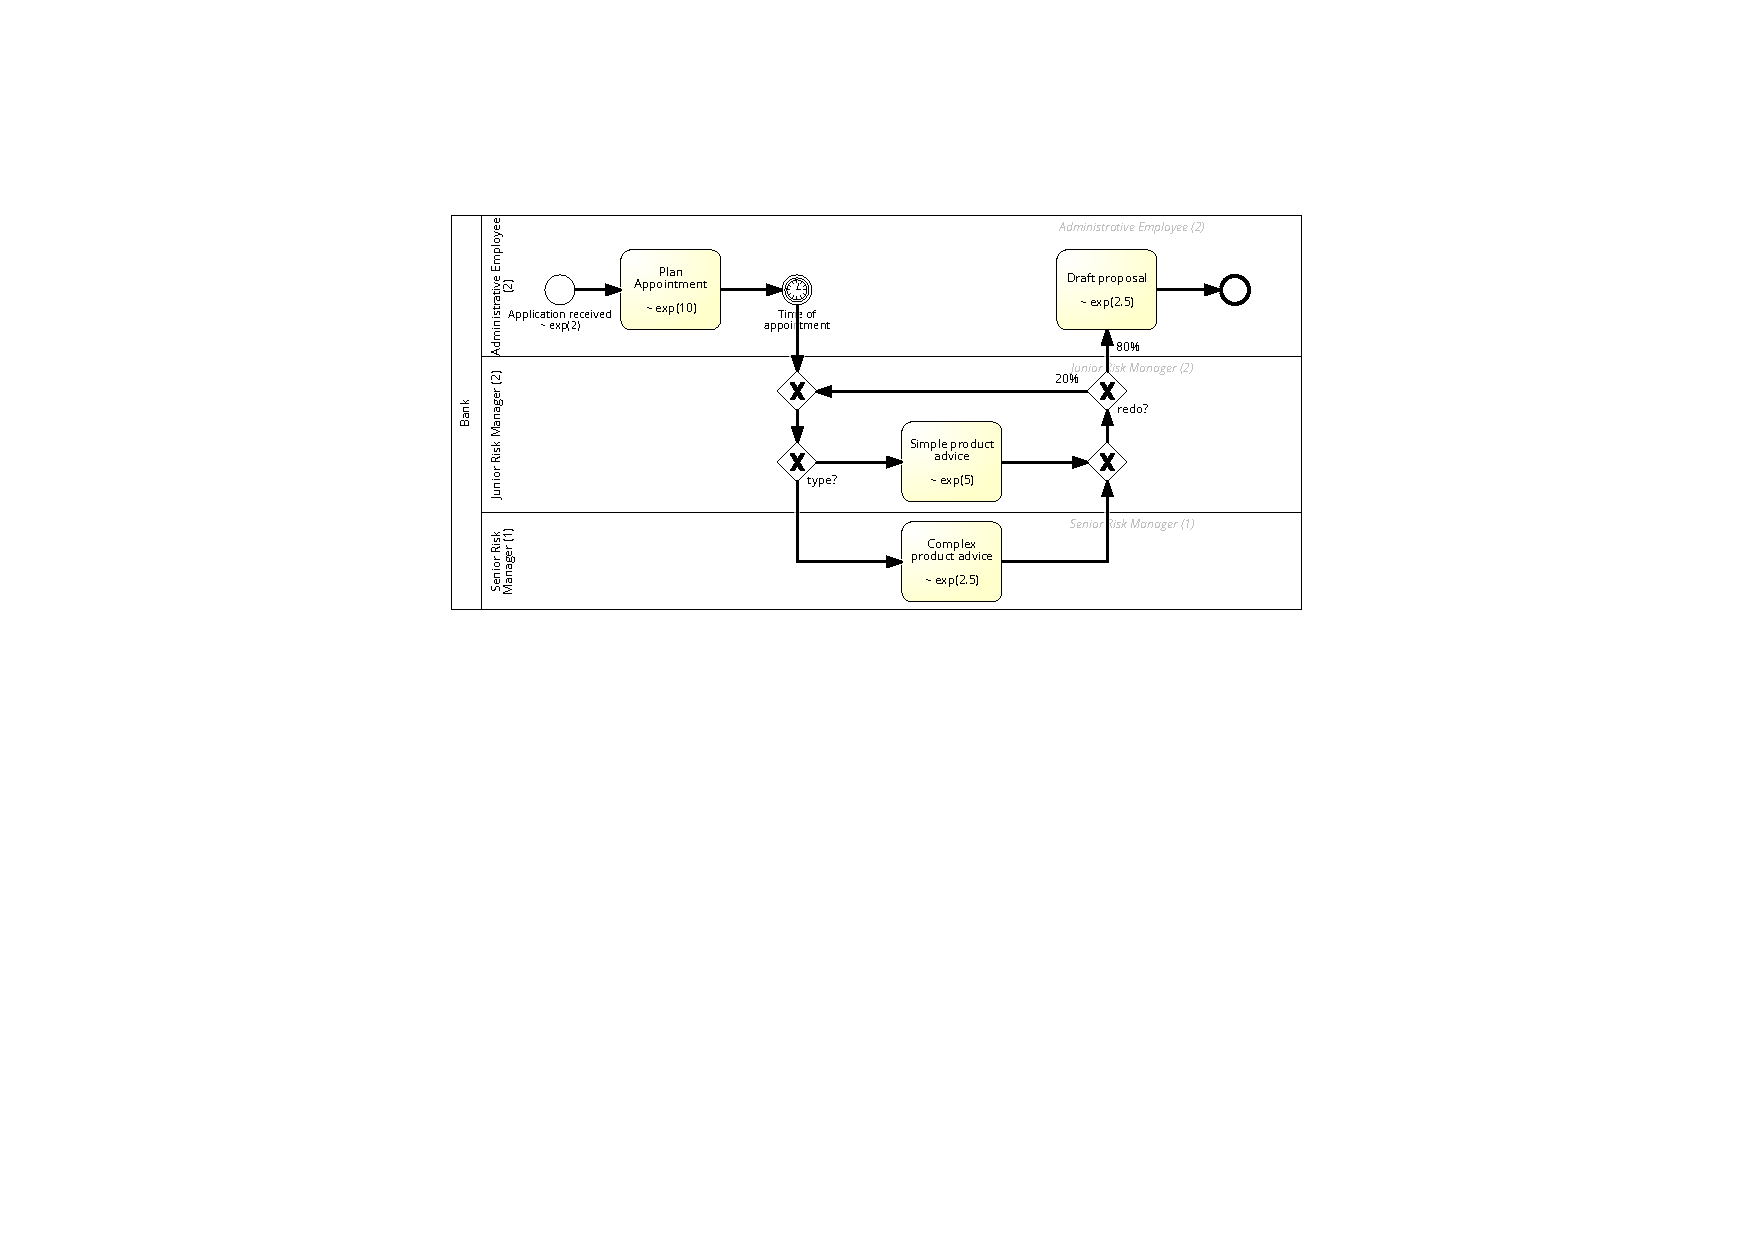
\includegraphics[width=0.98\textwidth,height=0.78\textheight,keepaspectratio]{process.pdf}
  \end{center}
  \vspace{-0.15cm}
  \smallref{A single BPMN model implies multiple decision points (admission, routing, rework, staffing).}
\end{frame}

% CORE
\begin{frame}{DayHospital is the archetype: high volume + high variability + high stakes}
  \begin{columns}[T]
    \column{0.62\textwidth}
      \begin{itemize}
        \item \btext{Many patients} per day; many activities; many resources
        \item \btext{Calendars}: shifts, partial capacity, vacations
        \item \btext{Uncertainty}: human-driven durations (heavy tails)
        \item \btext{Operational objective}: congestion and completion time
      \end{itemize}
      \vspace{0.2cm}
      \begin{block}{Running example across the talk}
        Same setting, three escalating non-locality mechanisms:
        \btext{robustness} \(\rightarrow\) \btext{learning mismatch} \(\rightarrow\) \btext{synchronization externalities}.
      \end{block}

    \column{0.38\textwidth}
      \centering
      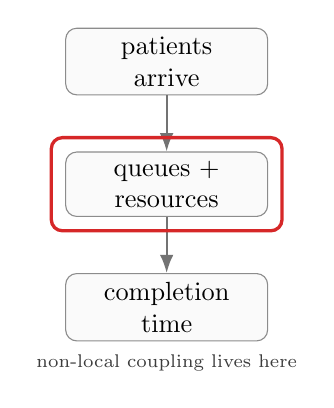
\begin{tikzpicture}[
        scale=0.95, every node/.style={transform shape},
        q/.style={rounded corners, draw=black!45, fill=black!2, minimum width=2.7cm, minimum height=0.8cm, align=center},
        arr/.style={-Latex, thick, draw=black!55}
      ]
        \node[q] (arrive) {patients\\arrive};
        \node[q, below=0.75cm of arrive] (queues) {queues +\\resources};
        \node[q, below=0.75cm of queues] (complete) {completion\\time};
        \draw[arr] (arrive) -- (queues);
        \draw[arr] (queues) -- (complete);
        \node[draw=badred, very thick, rounded corners, fit=(queues), inner sep=5pt] {};
        \node[below=0.05cm of complete, font=\scriptsize, color=darkgray] {non-local coupling lives here};
      \end{tikzpicture}
  \end{columns}

  \vspace{0.05cm}
  \smallref{Healthcare datasets in IJCAI'25 (BPSP) and IJCAI'26 (SASS) use DayHospital outpatient operations.}
\end{frame}

% CORE
\begin{frame}{Local dispatching is the wrong abstraction for BPO scheduling}
  \begin{block}{Local rule (what many systems implement)}
    Decide at each activity using only the local queue state (FIFO / SPT / static priorities).
  \end{block}
  \vspace{0.1cm}
  \begin{block}{What BPO actually optimizes}
    Process-level outcomes depend on downstream interactions:
    \begin{itemize}
      \item calendars couple decisions across \btext{time}
      \item uncertainty couples decisions across \btext{scenarios}
      \item gateways couple decisions across \btext{branches and cases}
    \end{itemize}
  \end{block}
  \vspace{0.15cm}
  \btext{This talk:} three progressively stronger fixes that all attack non-locality.
\end{frame}

% ==========================================================
% 2) Proactive scheduling (BPSP)
% ==========================================================
\section{1) Proactive scheduling under uncertainty and calendars (BPSP)}

% CORE
\begin{frame}{Goal: proactive schedules that remain good under uncertainty}
  \begin{block}{BPSP problem (informal)}
    Given a process model, resource calendars, and stochastic activity durations inferred from event logs,
    compute a schedule that minimizes a high-quantile (e.g., 95th percentile) completion time.
  \end{block}
  \vspace{0.2cm}
  \btext{Why this is already non-local:}
  uncertainty and calendars make decisions depend on future states and scenarios.
  \vspace{0.2cm}
  \smallref{Meneghello, Senderovich, Ronzani, Di Francescomarino, Ghidini, \emph{Proactive Data-driven Scheduling of Business Processes}, IJCAI 2025.}
\end{frame}

% CORE
\begin{frame}{Averages lie: logs give distributions, not constants}
  \begin{center}
    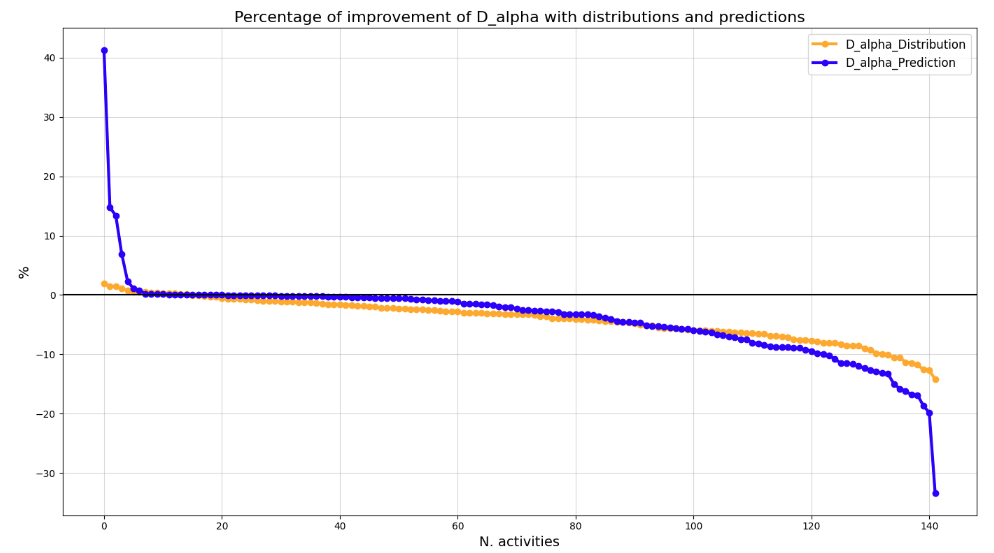
\includegraphics[width=0.95\textwidth,height=0.72\textheight,keepaspectratio]{distribution_predictions.png}
  \end{center}
  \vspace{-0.15cm}
  \smallref{Durations vary widely; robust objectives depend on distribution tails, not the mean.}
\end{frame}

% CORE (mandatory) — Gantt with calendar blocking
\begin{frame}{Calendars make feasibility non-local in time (vacations push work)}
  \begin{center}
    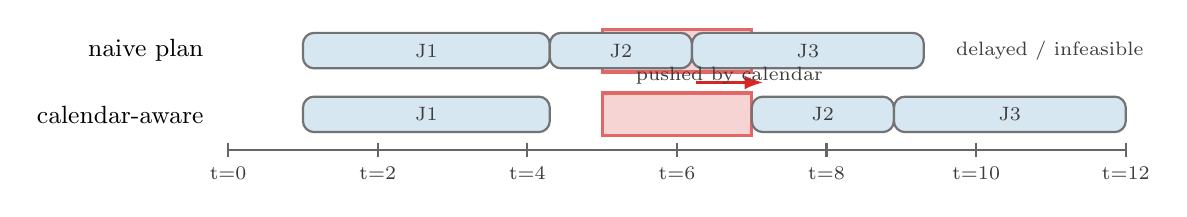
\begin{tikzpicture}[
      x=0.95cm, y=0.9cm,
      job/.style={rounded corners, draw=black!55, thick, fill=okblue!18, minimum height=0.55cm},
      vac/.style={draw=badred!70, very thick, fill=badred!20},
      axis/.style={draw=black!60, thick},
      lab/.style={font=\small},
      tiny/.style={font=\scriptsize, color=darkgray}
    ]
      \draw[axis] (0,0) -- (12,0);
      \foreach \t in {0,2,4,6,8,10,12} {
        \draw[axis] (\t,0.1) -- (\t,-0.1);
        \node[tiny, below] at (\t, -0.1) {t=\t};
      }

      \node[lab, anchor=east] at (-0.2, 1.4) {naive plan};
      \node[lab, anchor=east] at (-0.2, 0.5) {calendar-aware};

      \draw[vac] (5.0,1.1) rectangle (7.0,1.7);
      \node[tiny] at (6.0,1.4) {vacation};
      \draw[vac] (5.0,0.2) rectangle (7.0,0.8);

      \draw[job] (1.0,1.15) rectangle (4.3,1.65) node[midway,tiny]{J1};
      \draw[job] (4.3,1.15) rectangle (6.2,1.65) node[midway,tiny]{J2};
      \draw[job] (6.2,1.15) rectangle (9.3,1.65) node[midway,tiny]{J3};
      \node[tiny, anchor=west] at (9.6,1.4) {delayed / infeasible};

      \draw[job] (1.0,0.25) rectangle (4.3,0.75) node[midway,tiny]{J1};
      \draw[job] (7.0,0.25) rectangle (8.9,0.75) node[midway,tiny]{J2};
      \draw[job] (8.9,0.25) rectangle (12.0,0.75) node[midway,tiny]{J3};
      \draw[-Latex, thick, draw=badred] (6.25,0.95) -- (7.15,0.95);
      \node[tiny] at (6.7,1.05) {pushed by calendar};
    \end{tikzpicture}
  \end{center}
  \vspace{-0.1cm}
  \smallref{A local decision at \(t=4\) is constrained by a calendar event at \(t\in[5,7]\).}
\end{frame}

% CORE
\begin{frame}{BPSP is ``predict then optimize''—but with distributions and calendars}
  \begin{block}{From event logs to optimization parameters}
    \begin{itemize}
      \item estimate activity duration distributions \((\mu,\sigma)\) (possibly conditioned on features)
      \item estimate resource availability calendars
      \item infer precedence constraints from the process model
    \end{itemize}
  \end{block}
  \vspace{0.1cm}
  \btext{Key point:} naive point prediction (e.g., means) is insufficient for robust objectives.
\end{frame}

% CORE — pipeline diagram alone
\begin{frame}{BPSP solution is heavy because the objective is probabilistic}
  \begin{center}
    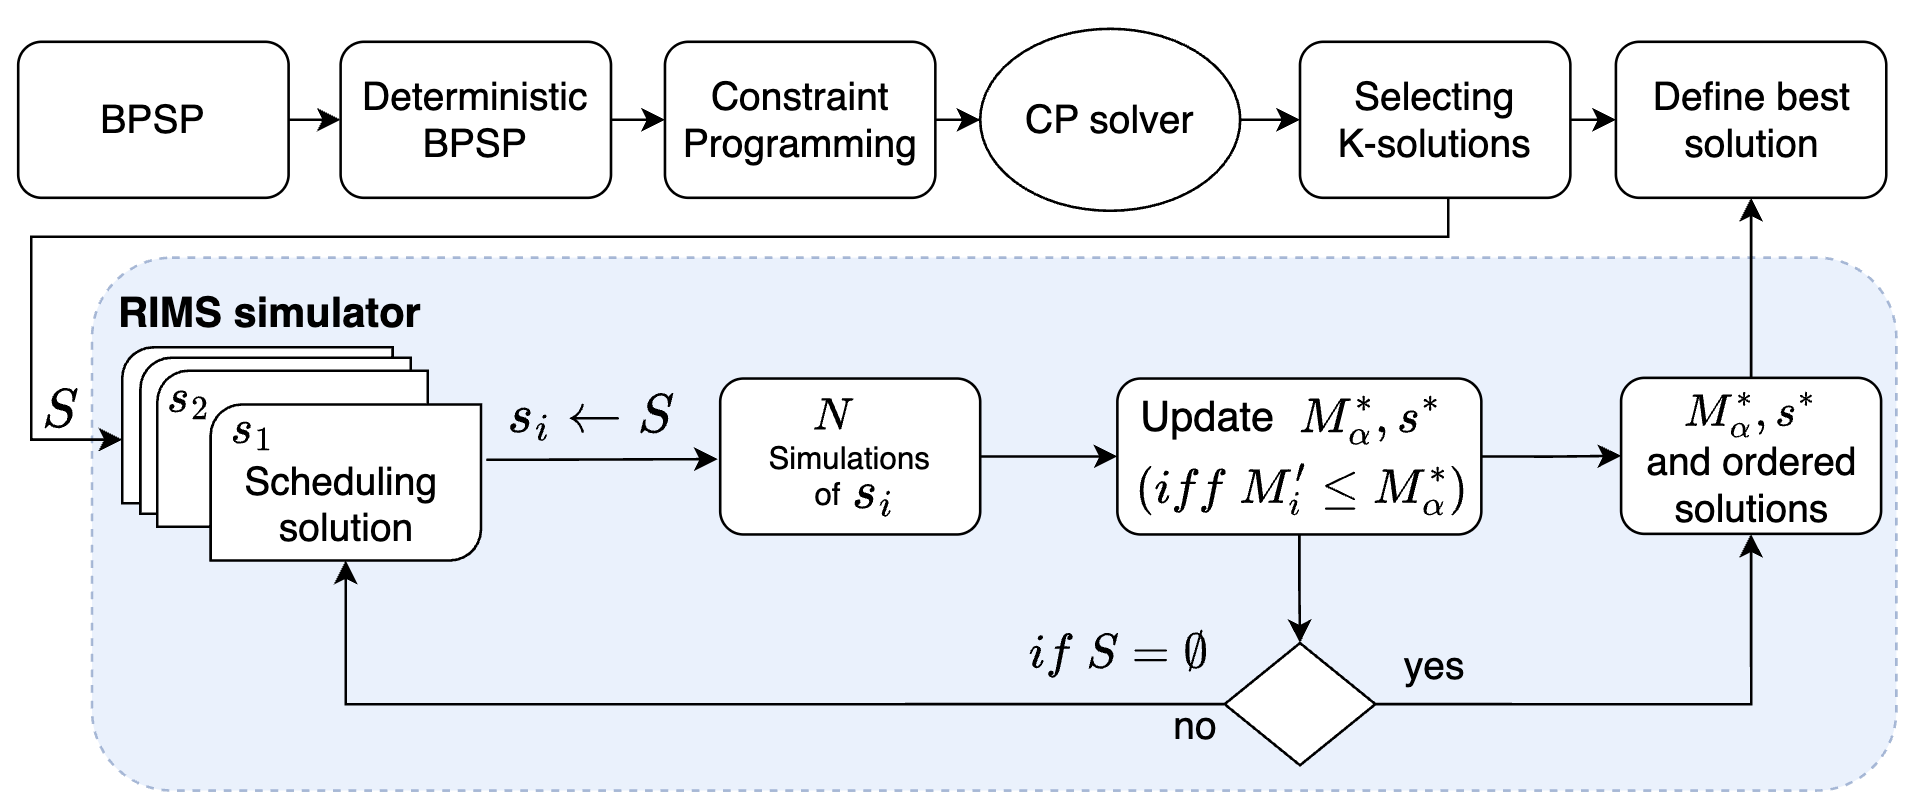
\includegraphics[width=0.98\textwidth,height=0.78\textheight,keepaspectratio]{pipeline_rims3.png}
  \end{center}
  \vspace{-0.15cm}
  \smallref{CP generates candidates; simulation evaluates robustness of candidates under stochastic durations.}
\end{frame}

% EXPAND — more formal BPSP statement
\iflong
% EXPAND
\begin{frame}{Formalizing BPSP: decision, feasibility, objective}
  \btext{Sets:}
  cases \(\mathcal{I}\), activities \(A_i\) per case, resources \(\mathcal{R}\).\\
  \btext{Precedence:} \(a_k \in \Pi_{i,a_j}\Rightarrow a_k \prec a_j\).\\
  \btext{Calendars:} \(v_{r,t}\in\{0,1\}\) availability of resource \(r\) at time \(t\).\\
  \btext{Random durations:} \(D_{i,a}\) with mean \(\mu_{i,a}\) and std \(\sigma_{i,a}\).

  \vspace{0.2cm}
  \btext{Objective (robust makespan):}
  \[
    M_\alpha^\star \;=\; \min_{s \in \mathcal{S}} \; \inf\left\{m:\Pr[M(s)\le m]\ge 1-\alpha\right\}.
  \]
  \smallref{Notation aligns with proactive scheduling; see Beck \& Wilson (2007) and IJCAI'25 BPSP paper.}
\end{frame}
\fi

% CORE (math, but light)
\begin{frame}{A principled buffer connects confidence to deterministic planning}
  \begin{block}{Buffered duration transform}
    Convert stochastic durations to deterministic ones:
    \[
      d_{i,a} \;=\; \mu_{i,a} \;+\; q \cdot \sigma_{i,a}.
    \]
  \end{block}
  \vspace{0.1cm}
  \begin{block}{Interpretation}
    \(q\) is an \btext{uncertainty coefficient}: larger \(q\) protects against the tail, at the cost of conservatism.
  \end{block}
  \smallref{Beck \& Wilson, \emph{Proactive Algorithms for Job Shop Scheduling with Probabilistic Durations}, JAIR 2007 (and related proactive scheduling work).}
\end{frame}

% EXPAND — theorem statement (more explicit)
\iflong
% EXPAND
\begin{frame}{Lower-bound theorem (proactive scheduling) — statement}
  \begin{block}{Theorem (informal, Beck \& Wilson style)}
    For confidence \(1-\alpha\), choosing
    \[
      q_U=\frac{\Phi^{-1}(1-\alpha)}{\sqrt{U}}
    \]
    yields a deterministic makespan \(M(q_U)\) that lower-bounds the probabilistic target \(M_\alpha^\star\),
    under standard assumptions (positive precedence expressions / critical-path bounding).
  \end{block}
  \begin{block}{Calendar extension (BPSP intuition)}
    Model vacations as fixed dummy intervals and express feasibility using precedence-style constraints;
    the PPE argument continues to apply.
  \end{block}
  \smallref{Beck \& Wilson (2007); BPSP extension: Meneghello et al., IJCAI 2025 (supplementary proof sketch).}
\end{frame}
\fi

% EXPAND — CP model details
\iflong
% EXPAND
\begin{frame}{CP model sketch: interval variables + calendars}
  \btext{Intervals:} for each activity \(a\) in case \(i\), interval \(x_{i,a}\) with start \(S(\cdot)\), length \(L(\cdot)\).\\
  \btext{Precedence:} \(\textsc{EndBeforeStart}(x_{i,a_k},x_{i,a_j})\) for all \(a_k\in\Pi_{i,a_j}\).\\
  \btext{Alternative resources:} choose one resource assignment among optional intervals.\\
  \btext{Calendars:} enforce \(\textsc{Unavailable}(x_{i,a,r}, v_{r,t})\).\\
  \btext{Capacity:} \(\textsc{Cumulative}(\cdot)\) constraints per resource.

  \vspace{0.15cm}
  \smallref{Implementation note: OR-Tools CP-SAT interval modeling; calendars as non-working windows.}
\end{frame}
\fi

% CORE
\begin{frame}{Result: proactive scheduling improves DayHospital makespan}
  \begin{block}{Empirical headline (IJCAI 2025)}
    Average makespan improvement: \btext{5\%--14\%} on real hospital days (up to \(\sim\)4 hours on busy days).
  \end{block}
  \vspace{0.2cm}
  \begin{center}
    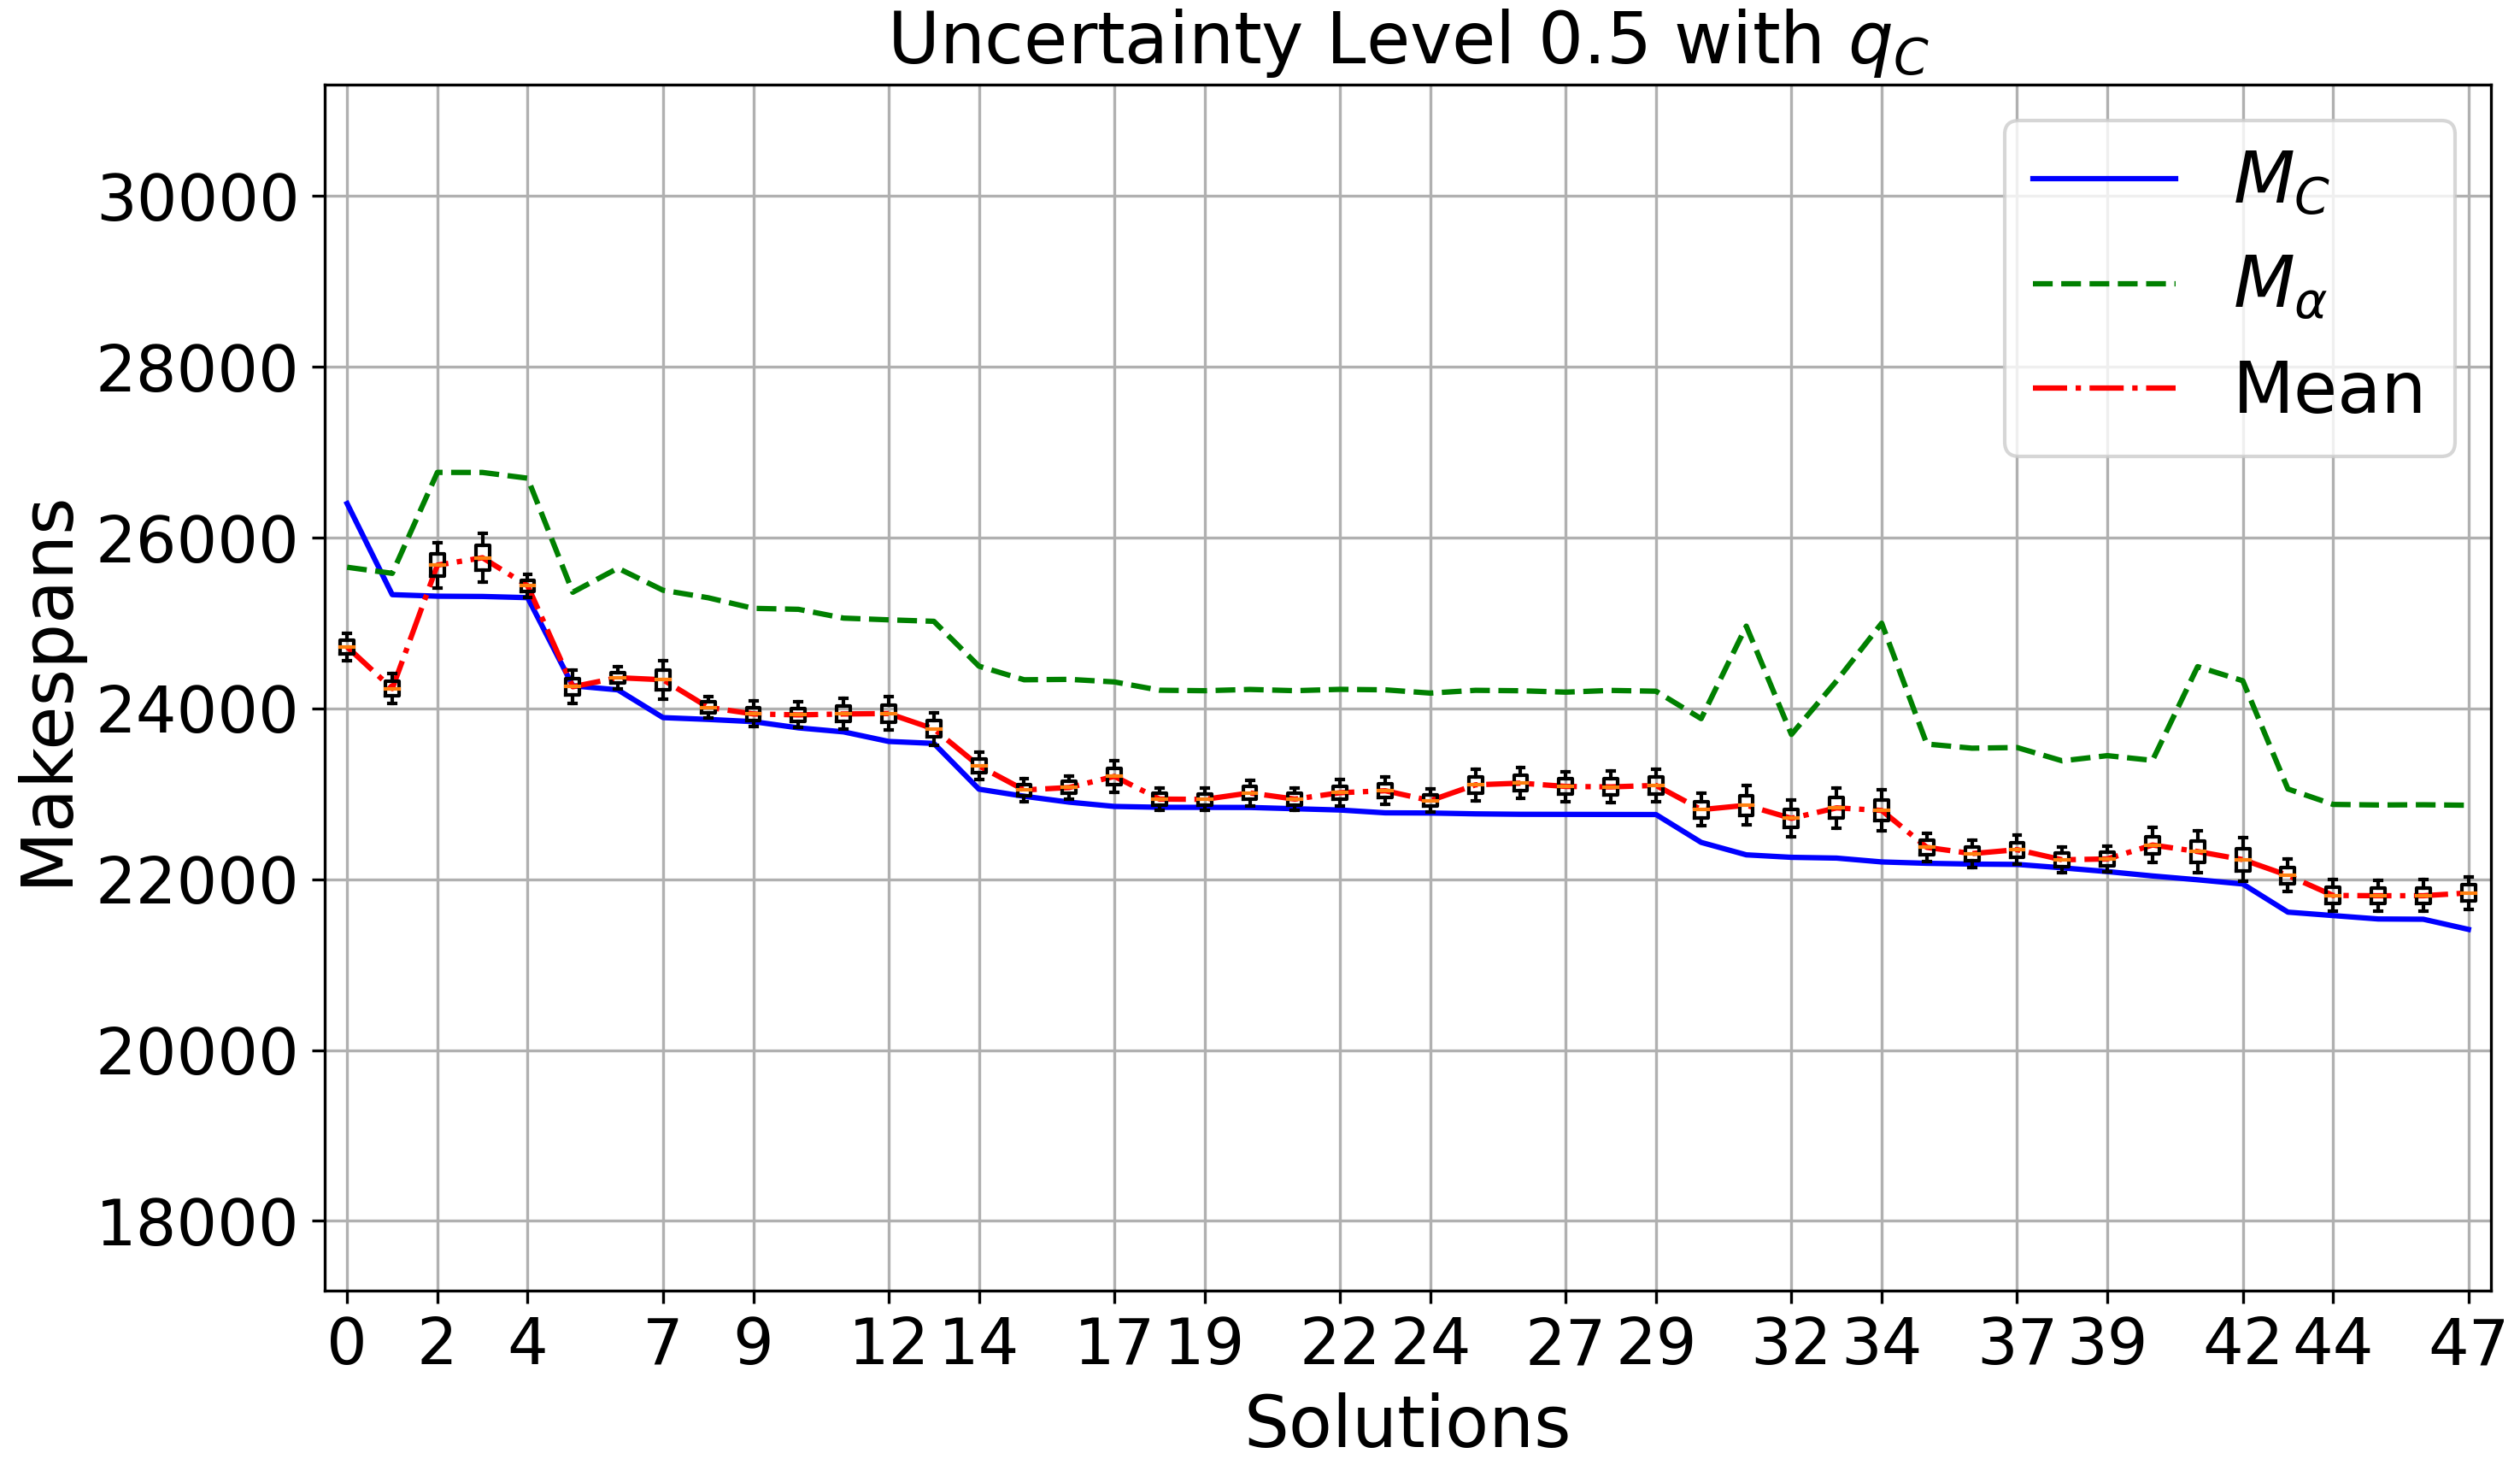
\includegraphics[width=0.75\textwidth]{uncertainty_caledars_2.png}
  \end{center}
  \vspace{-0.15cm}
  \smallref{Deterministic vs probabilistic performance across candidate schedules (q-choices trade off guarantee vs tightness).}
\end{frame}

% CORE (transition)
\begin{frame}{Transition: can we avoid heavy CP + simulation?}
  \begin{block}{What BPSP solves}
    Robustness to uncertainty + calendar feasibility for a centralized planner.
  \end{block}
  \vspace{0.1cm}
  \begin{block}{What it costs}
    Global optimization (\btext{CP}) + probabilistic evaluation (\btext{Monte Carlo simulation}) is heavy.
  \end{block}
  \vspace{0.15cm}
  \btext{Next move:} focus on settings where the deterministic optimum is a \btext{polynomial-time rule}, so optimization is cheap—then fix the learning objective.
\end{frame}

% ==========================================================
% 3) SASS — learning to schedule without CP/simulation
% ==========================================================
\section{2) Learning to schedule without CP/simulation (SASS)}

% CORE
\begin{frame}{Key idea: exploit polynomial-time scheduling structure}
  \begin{block}{Surrogate-friendly scheduling problems}
    Deterministic optimum is given by a known polynomial-time rule \(\mathcal{A}\)
    (e.g., SPT, Johnson).
  \end{block}
  \vspace{0.15cm}
  \begin{block}{Why this matters}
    At inference, scheduling is cheap: \(\hat{\pi} = \mathcal{A}(\hat{\theta})\).
    The challenge becomes: \btext{learn predictions that produce good schedules}.
  \end{block}
  \smallref{SASS paper: ``SASS: Structure-Aware Surrogates for Learning to Schedule'', IJCAI 2026 submission (current draft in repo).}
\end{frame}

% CORE
\begin{frame}{MSE is misaligned: scheduling depends on discrete critical decisions}
  \begin{block}{Predict-then-optimize baseline}
    Train \(\hat{\theta}=f_\omega(x)\) by MSE, then schedule by \(\mathcal{A}(\hat{\theta})\).
  \end{block}
  \vspace{0.15cm}
  \btext{Failure mode:} a small numeric error flips a comparison \(\Rightarrow\) a different schedule.
  \vspace{0.15cm}
  \smallref{Decision-focused learning: Elmachtoub \& Grigas, \emph{Smart ``Predict, then Optimize''}, Management Science 2022 (and SPO+ variants).}
\end{frame}

% CORE (mandatory) — swap cartoon
\begin{frame}{Swap-cost intuition: tiny error \(\Rightarrow\) flipped order \(\Rightarrow\) regret}
  \begin{columns}[T]
    \column{0.52\textwidth}
      \btext{True}: \(y_A<y_B\) \(\Rightarrow\) SPT serves \(A\) before \(B\).\\
      \vspace{0.2cm}
      
\begin{tikzpicture}[x=0.42cm,y=0.9cm,
        job/.style={rounded corners, draw=black!55, thick, fill=okblue!18, minimum height=0.55cm},
        tiny/.style={font=\scriptsize, color=darkgray}]
        \node[tiny, anchor=west] at (0,1.05) {correct order};
        \draw[job] (0,0.35) rectangle (10,0.85) node[midway,tiny]{A};
        \draw[job] (10,0.35) rectangle (21,0.85) node[midway,tiny]{B};
      \end{tikzpicture}

    \column{0.48\textwidth}
      \btext{Predicted}: \(\hat{y}_A>\hat{y}_B\) flips the pair.\\
      \vspace{0.2cm}
      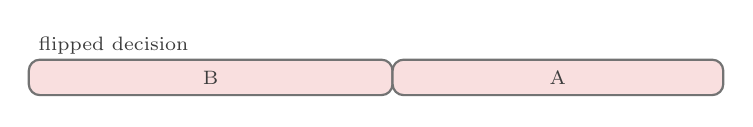
\begin{tikzpicture}[x=0.42cm,y=0.9cm,
        job/.style={rounded corners, draw=black!55, thick, fill=badred!15, minimum height=0.55cm},
        tiny/.style={font=\scriptsize, color=darkgray}]
        \node[tiny, anchor=west] at (0,1.05) {flipped decision};
        \draw[job] (0,0.35) rectangle (11,0.85) node[midway,tiny]{B};
        \draw[job] (11,0.35) rectangle (21,0.85) node[midway,tiny]{A};
      \end{tikzpicture}
  \end{columns}
  \vspace{0.15cm}
  \btext{Takeaway:} the loss should target \emph{critical decisions}, weighted by their downstream cost.
\end{frame}

% CORE (requested) — four steps diagram
\begin{frame}{SASS is a 4-step recipe (decision structure \(\rightarrow\) differentiable training)}
  \begin{center}
    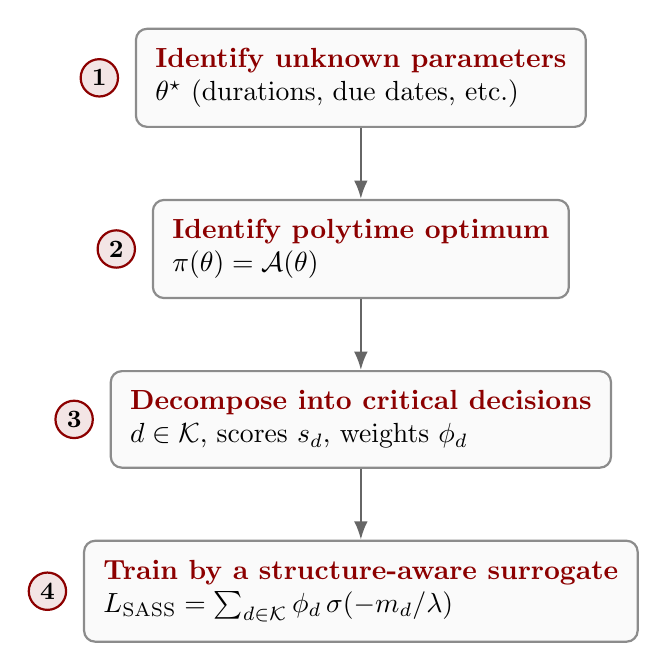
\begin{tikzpicture}[
      node distance=0.9cm and 1.0cm,
      box/.style={rounded corners, draw=black!45, thick, fill=black!2, inner sep=7pt, align=left},
      num/.style={circle, draw=darkred, thick, fill=darkred!10, inner sep=2pt, font=\bfseries\small},
      arr/.style={-Latex, thick, draw=black!60}
    ]
      \node[box] (s1) {\btext{Identify unknown parameters}\\\(\theta^\star\) (durations, due dates, etc.)};
      \node[box, below=of s1] (s2) {\btext{Identify polytime optimum}\\\(\pi(\theta)=\mathcal{A}(\theta)\)};
      \node[box, below=of s2] (s3) {\btext{Decompose into critical decisions}\\\(d\in\mathcal{K}\), scores \(s_d\), weights \(\phi_d\)};
      \node[box, below=of s3] (s4) {\btext{Train by a structure-aware surrogate}\\\(L_{\mathrm{SASS}}=\sum_{d\in\mathcal{K}}\phi_d\,\sigma(-m_d/\lambda)\)};

      \node[num, left=0.2cm of s1.west] {1};
      \node[num, left=0.2cm of s2.west] {2};
      \node[num, left=0.2cm of s3.west] {3};
      \node[num, left=0.2cm of s4.west] {4};

      \draw[arr] (s1) -- (s2);
      \draw[arr] (s2) -- (s3);
      \draw[arr] (s3) -- (s4);
    \end{tikzpicture}
  \end{center}
  \vspace{0.1cm}
  \smallref{SASS: Structure-Aware Surrogates for Learning to Schedule, IJCAI 2026 submission (current draft).}
\end{frame}

% CORE — general math
\begin{frame}{Math: regret is non-differentiable; SASS builds a differentiable surrogate}
  \btext{Regret (general):}
  \[
    R(\hat{\theta},\theta^\star)
    \;=\;
    C(\pi(\hat{\theta});\theta^\star)\;-\;C(\pi(\theta^\star);\theta^\star),
  \]
  where \(\pi(\theta)=\mathcal{A}(\theta)\) is a discrete rule.

  \vspace{0.15cm}
  \btext{SASS surrogate:}
  \[
    L_{\mathrm{SASS}}(\omega)
    \;=\;
    \sum_{d\in\mathcal{K}}
      \phi_d(\theta^\star)\,
      \sigma\!\left(\frac{-m_d(\omega;x,\theta^\star)}{\lambda}\right).
  \]

  \vspace{0.1cm}
  \smallref{\(\mathcal{K}\)=critical decisions; \(m_d\)=oriented margin (correct iff \(m_d>0\)); \(\phi_d\)=local objective impact.}
\end{frame}

% CORE — instantiate SCT/SPT with full math
\begin{frame}{Instantiation (Problem 1): single-machine SCT with SPT}
  \btext{Deterministic optimum:} SPT sorts by true processing times \(y_i\).\\
  \btext{Objective:} minimize sum of completion times (SCT).

  \vspace{0.15cm}
  \btext{Swap cost (true impact):}
  swapping two tasks at positions \(i<j\) changes SCT by
  \[
    R_{i,j} = (j-i)(y_j-y_i).
  \]

  \vspace{0.1cm}
  \btext{SASS loss for SCT (sigmoid pairwise):}
  \[
    L_{\mathrm{SCT}}(\omega)=
    \sum_{y_i<y_j}
      R_{i,j}\,
      \sigma\!\left(\frac{f_\omega(x_i)-f_\omega(x_j)}{\lambda}\right).
  \]
  \smallref{Matches the current SASS draft (\texttt{IJCAI2026\_Learn\_to\_Schedule/main.tex}).}
\end{frame}

% EXPAND — Johnson math (second problem)
\iflong
% EXPAND
\begin{frame}{Instantiation (Problem 2): flow shop makespan via Johnson’s rule}
  \btext{Deterministic optimum:} Johnson partitions jobs into
  \(G_1=\{i:p_{i1}<p_{i2}\}\), \(G_2=\{i:p_{i1}\ge p_{i2}\}\),
  orders \(G_1\) ascending by \(p_{i1}\), orders \(G_2\) descending by \(p_{i2}\).

  \vspace{0.15cm}
  \btext{Critical decisions:}
  (i) correct group assignment, (ii) correct ordering inside each group.

  \vspace{0.1cm}
  \btext{SASS structure:}
  two surrogate components \(L_{\mathrm{group}}+L_{\mathrm{order}}\),
  each weighted by makespan-impact terms (swap costs / distance-to-boundary).

  \smallref{See SASS draft Section ``Problem 2: Flow Shop Scheduling''.}
\end{frame}
\fi

% CORE — synthetic evidence (split; keep one for TU/e, two for TUM)
\begin{frame}{Evidence: SASS is stable where SPO+ becomes brittle (synthetic)}
  \begin{center}
    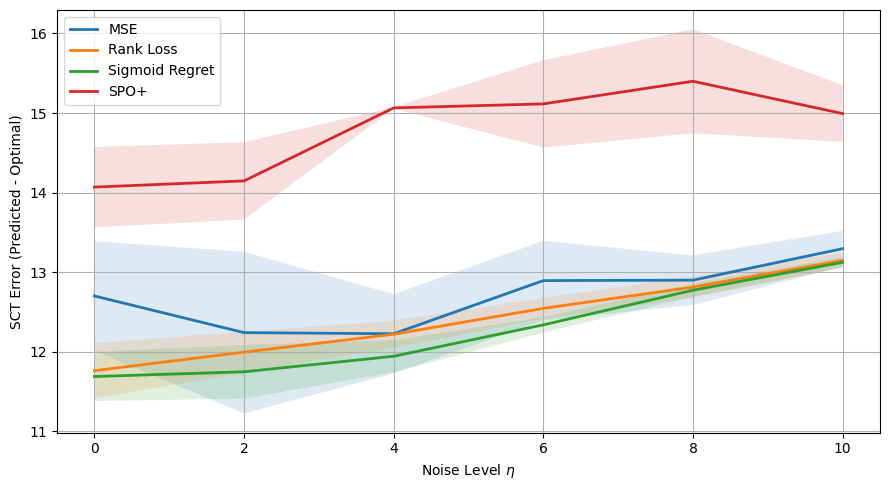
\includegraphics[width=0.95\textwidth,height=0.72\textheight,keepaspectratio]{linearDataset_problem1.png}
  \end{center}
  \vspace{-0.15cm}
  \smallref{Relative SCT error vs optimal schedule on synthetic linear datasets (SASS vs baselines).}
\end{frame}

\iflong
% EXPAND
\begin{frame}{Evidence: sampled pairs are enough for scalability}
  \begin{center}
    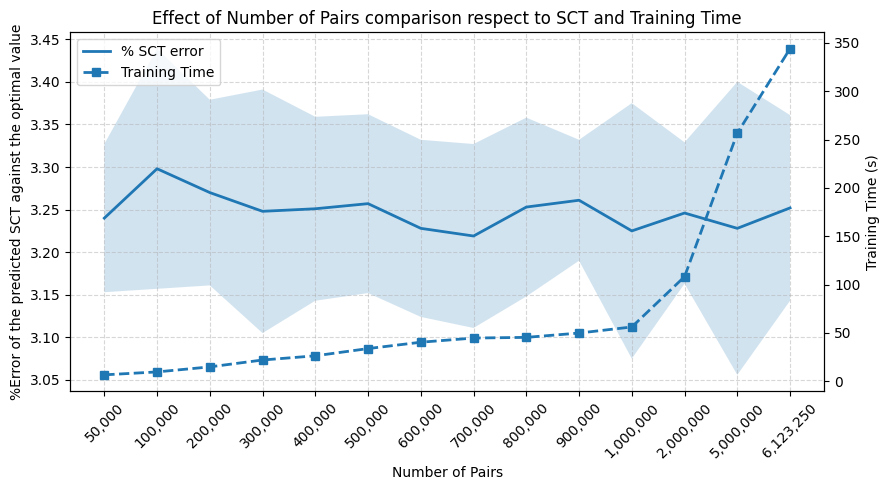
\includegraphics[width=0.95\textwidth,height=0.72\textheight,keepaspectratio]{analysis_number_of_pairs.png}
  \end{center}
  \vspace{-0.15cm}
  \smallref{SASS scales by sampling a subset of job pairs (e.g., \(\sim10{,}000\) pairs already works well).}
\end{frame}
\fi

% CORE — DayHospital results (complete, no placeholders)
\begin{frame}{DayHospital: SASS improves schedules (Jan--Dec 2021)}
  \begin{columns}[T]
    \column{0.58\textwidth}
      \begin{block}{Metric: average relative SCT error vs optimal ordering}
        \vspace{-0.1cm}
        \begin{table}
          \small
          \setlength{\tabcolsep}{6pt}
          \renewcommand{\arraystretch}{1.15}
          \begin{tabular}{l c}
            \toprule
            Method & Avg.\ rel.\ SCT error \\
            \midrule
            \btext{SASS (ours)} & \btext{0.316} \\
            Predict-then-optimize (MSE) & 0.353 \\
            Learn-to-rank (LTR) & 0.338 \\
            SPO+ & 0.476 \\
            \bottomrule
          \end{tabular}
        \end{table}
      \end{block}
      \vspace{0.05cm}
      \btext{Key claim:} improving schedule quality requires decision-aware training, not MSE.

    \column{0.42\textwidth}
      \centering
      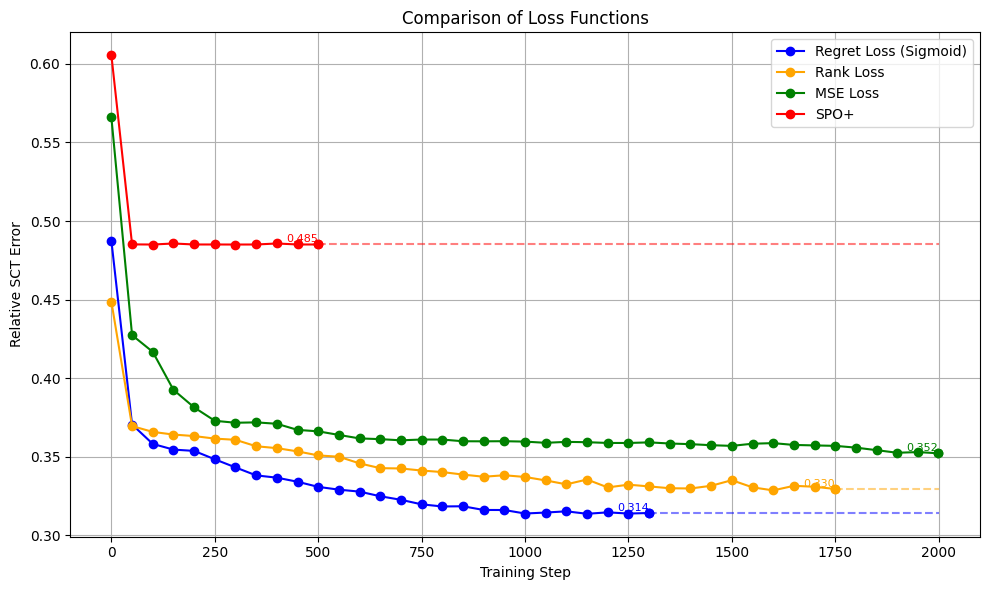
\includegraphics[width=0.95\textwidth,height=0.62\textheight,keepaspectratio]{LossComparison_Jan.png}
      \vspace{0.05cm}
      \smallref{Training dynamics (Jan 2021).}
  \end{columns}
\end{frame}

% CORE (transition to valuation)
\begin{frame}{Transition: BPSP and SASS still assume one controller}
  \begin{block}{What we fixed so far}
    \begin{itemize}
      \item BPSP: robust planning under uncertainty + calendars (heavy CP + simulation)
      \item SASS: avoid CP/simulation by exploiting polytime rules + decision-aware learning
    \end{itemize}
  \end{block}
  \vspace{0.1cm}
  \begin{block}{What remains (and why this is still BPO)}
    Real processes contain fork--join structures where \btext{synchronization creates externalities}.
    Cases (patients/jobs) may effectively ``compete'' for coordinated progress.
  \end{block}
  \vspace{0.1cm}
  \btext{Next:} locality fails even with good predictions—because incentives and synchronization are non-local.
\end{frame}

% ==========================================================
% 4) Valuation and synchronization externalities (capstone)
% ==========================================================
\section{3) Fork--join synchronization creates externalities (valuation capstone)}

% CORE — OR example
\begin{frame}{Claim: FIFO is locally fair but globally inefficient at OR joins}
  \begin{columns}[T]
    \column{0.55\textwidth}
      \centering
      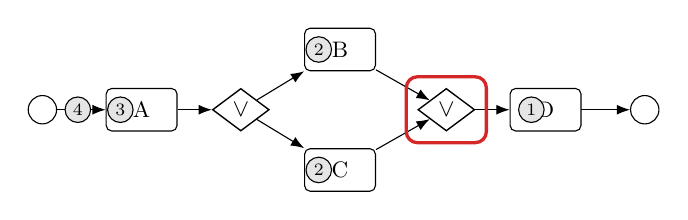
\begin{tikzpicture}[
        scale=0.9, every node/.style={transform shape},
        >=Latex,
        event/.style={circle,draw,minimum size=4mm},
        gateway/.style={diamond,draw,aspect=2.4,minimum width=8mm,minimum height=6mm,inner sep=0pt,line width=0.5pt},
        activity/.style={rectangle,draw,rounded corners=2pt,minimum width=10mm,minimum height=6mm,font=\small},
        case/.style={circle,draw,fill=black!10,inner sep=0.5pt,minimum size=3.6mm,font=\scriptsize}
      ]
        \node[event]    (start) at (0,0) {};
        \node[activity] (A)     at (1.4,0) {A};
        \node[gateway]  (split) at (2.8,0) {};
        \node[activity] (B)     at (4.2,0.85) {B};
        \node[activity] (C)     at (4.2,-0.85) {C};
        \node[gateway]  (join)  at (5.7,0) {};
        \node[activity] (D)     at (7.1,0) {D};
        \node[event]    (end)   at (8.5,0) {};
        \node at (split.center) {$\vee$};
        \node at (join.center)  {$\vee$};
        \draw[->] (start) -- (A);
        \draw[->] (A) -- (split);
        \draw[->] (split) -- (B);
        \draw[->] (split) -- (C);
        \draw[->] (B) -- (join);
        \draw[->] (C) -- (join);
        \draw[->] (join) -- (D);
        \draw[->] (D) -- (end);

        % cases (visual cue)
        \node[case] at (6.9, 0.00) {1};
        \node[case] at (3.9, 0.85) {2};
        \node[case] at (3.9,-0.85) {2};
        \node[case] at (1.1, 0.00) {3};
        \node[case] at (0.5, 0.00) {4};
        \node[draw=badred, very thick, rounded corners, fit=(join), inner sep=4pt] {};
      \end{tikzpicture}
      \vspace{0.05cm}
      \smallref{OR join couples queues \(B\) and \(C\).}

    \column{0.45\textwidth}
      \begin{block}{Externality}
        Serving a case at \(B\) changes waiting at the join, affecting completion times of other cases.
      \end{block}
      \begin{block}{Non-locality}
        A local scheduling decision changes global flow via synchronization.
      \end{block}
  \end{columns}
  \vspace{0.05cm}
  \smallref{Valuation paper draft: \emph{Valuation-Driven Scheduling in Business Processes}, IJCAI 2026 submission.}
\end{frame}

% CORE for TU/e: stop valuation here (at most one intuition slide)
\iflong\else
% CORE
\begin{frame}{TU/e takeaway: fork--join makes ``fair'' local rules globally wrong}
  \begin{block}{One-sentence conclusion}
    Synchronization introduces \btext{delay externalities} that cannot be fixed by tuning local priorities.
  \end{block}
  \vspace{0.15cm}
  \btext{TUM extension:} valuation-aware scheduling internalizes these externalities via pricing.
\end{frame}
\fi

% EXPAND — valuation as climax (TUM)
\iflong
% EXPAND
\begin{frame}{Value-of-time is a compact signal for non-local delay costs}
  \begin{block}{Model}
    Each case \(i\) reports a value-of-time function \(v_i(t)\) (marginal cost of waiting).
  \end{block}
  \vspace{0.1cm}
  \begin{block}{Welfare objective (sketch)}
    Choose a scheduling policy that maximizes aggregate reported welfare (generalizes weighted flow time).
  \end{block}
  \vspace{0.15cm}
  \begin{columns}[T]
    \column{0.55\textwidth}
      \btext{Intuition:} \(v_i(t)\) implicitly encodes preferences over bundles of queue positions across required branches.
    \column{0.45\textwidth}
      \centering
      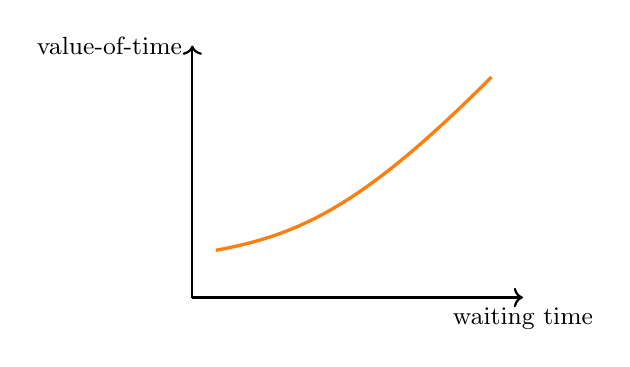
\begin{tikzpicture}[x=1.0cm,y=1.0cm]
        \draw[->, thick] (0,0) -- (4.2,0) node[below, font=\small]{waiting time};
        \draw[->, thick] (0,0) -- (0,3.2) node[left, font=\small]{value-of-time};
        \draw[very thick, color=okorange] (0.3,0.6) .. controls (1.4,0.8) and (2.2,1.2) .. (3.8,2.8);
      \end{tikzpicture}
  \end{columns}
  \smallref{Mechanism-design background: Nisan et al., \emph{Algorithmic Game Theory}, 2007 (VCG); classic VCG: Vickrey 1961; Clarke 1971; Groves 1973.}
\end{frame}

% EXPAND
\begin{frame}{VCG-style payments price delay externalities (why ``efficiency vs fairness'' is a false dichotomy)}
  \btext{Setup:} reported welfare \(W(\cdot)\) induced by schedules. Let \(s^\star\) maximize welfare.
  \vspace{0.1cm}

  \btext{VCG payment (canonical form):}
  \[
    p_i \;=\; \max_{s} W_{-i}(s)\;-\;W_{-i}(s^\star),
  \]
  where \(W_{-i}\) excludes case \(i\)'s reported value.

  \vspace{0.1cm}
  \begin{block}{Interpretation}
    Case \(i\) pays exactly the harm (delay externality) it imposes on others.
    FIFO is a \btext{baseline} (zero pricing), not the objective.
  \end{block}
  \smallref{Valuation paper draft: ``FIFO emerges as baseline; deviations regulated by VCG-style payments.''}
\end{frame}

% EXPAND
\begin{frame}{Climax: valuation is the unifier of non-locality in BPO scheduling}
  \begin{itemize}
    \item BPSP: handles non-locality across \btext{time} and \btext{scenarios} (calendars + uncertainty)
    \item SASS: handles non-locality inside the \btext{learning objective} (critical decisions, swap costs)
    \item Valuation: handles non-locality across \btext{cases and branches} (externalities + incentives)
  \end{itemize}
  \vspace{0.15cm}
  \begin{block}{Single thesis, now complete}
    Scheduling in business processes is fundamentally non-local; valuation makes the non-local costs explicit and actionable.
  \end{block}
\end{frame}
\fi

% ==========================================================
% 5) Synthesis / agenda
% ==========================================================
\section{Synthesis \& research agenda}

% CORE
\begin{frame}{Structure-aware BPO: logs \(\rightarrow\) robustness \(\rightarrow\) learning \(\rightarrow\) incentives}
  \begin{center}
    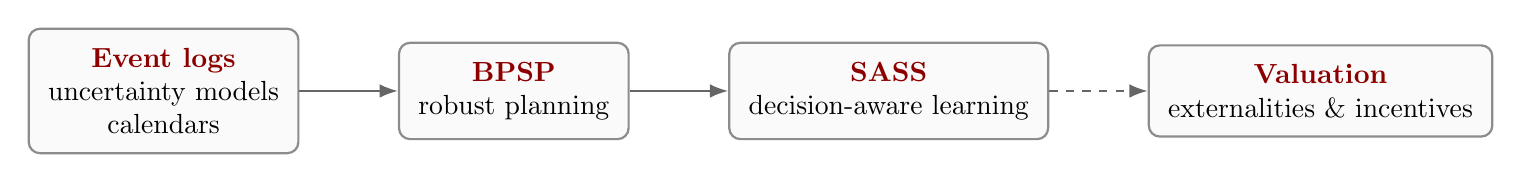
\begin{tikzpicture}[
      node distance=0.95cm and 1.25cm,
      box/.style={rounded corners, draw=black!45, thick, fill=black!2, inner sep=7pt, align=center},
      arr/.style={-Latex, thick, draw=black!60}
    ]
      \node[box] (logs) {\btext{Event logs}\\uncertainty models\\calendars};
      \node[box, right=of logs] (b) {\btext{BPSP}\\robust planning};
      \node[box, right=of b] (s) {\btext{SASS}\\decision-aware learning};
      \node[box, right=of s] (v) {\btext{Valuation}\\externalities \& incentives};
      \draw[arr] (logs) -- (b);
      \draw[arr] (b) -- (s);
      \iflong
        \draw[arr] (s) -- (v);
      \else
        \draw[arr, dashed] (s) -- (v);
      \fi
    \end{tikzpicture}
  \end{center}
  \vspace{0.15cm}
  \btext{Agenda:} unify process mining + robust optimization + decision-focused learning + mechanism design for BPO control.
\end{frame}

% CORE
\begin{frame}{Key references (exact)}
  \scriptsize
  \begin{itemize}
    \item Dumas, La Rosa, Mendling, Reijers. \emph{Fundamentals of Business Process Management}. Springer, 2nd ed., 2018.
    \item Beck, Wilson. \emph{Proactive Algorithms for Job Shop Scheduling with Probabilistic Durations}. Journal of Artificial Intelligence Research (JAIR), 2007.
    \item Meneghello, Senderovich, Ronzani, Di Francescomarino, Ghidini. \emph{Proactive Data-driven Scheduling of Business Processes}. IJCAI, 2025.
    \item Elmachtoub, Grigas. \emph{Smart ``Predict, then Optimize''}. Management Science, 2022.
    \item (SASS draft) \emph{SASS: Structure-Aware Surrogates for Learning to Schedule}. IJCAI 2026 submission (current repo version).
    \item (Valuation draft) \emph{Valuation-Driven Scheduling in Business Processes}. IJCAI 2026 submission (current repo version).
    \item Vickrey (1961), Clarke (1971), Groves (1973). VCG mechanisms (canonical foundations); see Nisan et al., \emph{Algorithmic Game Theory}, 2007.
  \end{itemize}
\end{frame}

% CORE
\begin{frame}{Closing claim: locality is the default mistake in BPO scheduling}
  \begin{enumerate}
    \item \btext{Non-locality is structural}: calendars, uncertainty, gateways.
    \item \btext{BPSP} makes uncertainty operational (robust plans; heavy but principled).
    \item \btext{SASS} aligns learning with schedule quality (polytime structure; swap-cost surrogates).
    \item \iflong\btext{Valuation} internalizes externalities (synchronization + incentives) as the capstone.\else\btext{Valuation} is the next step when synchronization creates externalities.\fi
  \end{enumerate}
  \vspace{0.25cm}
  \btext{Thank you.}
\end{frame}

% ==========================================================
% Appendix (extra math / details)
% ==========================================================
\appendix
\section{Appendix}

% APPENDIX
\begin{frame}{Appendix: CP constraints (BPSP) — more detail}
  \scriptsize
  \begin{itemize}
    \item Interval vars \(x_{i,a}\); optional assignment intervals \(\bar{x}_{i,a,r}\)
    \item \(\textsc{Alternative}(x_{i,a}, \{\bar{x}_{i,a,r}\}_{r\in R(a)})\)
    \item \(\textsc{EndBeforeStart}(x_{i,a_k},x_{i,a_j})\) for precedence
    \item \(\textsc{Unavailable}(\bar{x}_{i,a,r}, v_{r,t})\) for calendars
    \item \(\textsc{Cumulative}(\{\bar{x}_{i,a,r}\}, C_r)\) for capacity
  \end{itemize}
  \smallref{Matches the IJCAI'25 BPSP method section (CP + simulation selection).}
\end{frame}

% APPENDIX
\begin{frame}{Appendix: oriented margins and decision weights (SASS) — more detail}
  \scriptsize
  \btext{Decision score} \(s_d(\omega;x)\) produces a sign;\\
  \btext{Oriented margin} \(m_d(\omega;x,\theta^\star)\) is positive iff the decision is correct.\\
  \btext{Weight} \(\phi_d(\theta^\star)\ge 0\) equals the objective impact of getting decision \(d\) wrong.\\
  \[
    L_{\mathrm{SASS}}(\omega)
    =
    \sum_{d\in\mathcal{K}}
      \phi_d(\theta^\star)\,
      \sigma\!\left(\frac{-m_d(\omega;x,\theta^\star)}{\lambda}\right).
  \]
  \smallref{See SASS draft Section ``Surrogate-Based Predict-and-Schedule'' for the full formalism.}
\end{frame}

\end{document}

